\subsubsection{Reconstruction et ajustement des arbres de phages}
La collection réunit la référence du phage \(\phi\)X174 (\texttt{NC\_001422.1}) et 63 autres génomes complets obtenus avec NCBI Datasets~18.41.1~\cite{phixref,ncbidatasets}. Chaque génome est identifié par son accession versionnée, sa longueur et son empreinte SHA-256. L’ajustement se mesure par l’écart entre la distance d’édition de deux génomes et la longueur du chemin entre leurs feuilles. Une origine différente sur le génome circulaire peut modifier la distance entre les chaînes déposées. Une même édition observée peut aussi résulter de plusieurs événements évolutifs.

UPGMA, la méthode de classification moyenne de Sokal et Michener~\cite{upgma}, joint les groupes \(U,V\) de distance moyenne minimale et place leur parent à la hauteur \(d(U,V)/2\). Pour un troisième groupe \(W\), la nouvelle distance moyenne est pondérée par les effectifs. Saitou et Nei ont proposé Neighbor-Joining (NJ) pour construire un arbre non enraciné~\cite{nj}. NJ joint la paire qui minimise \(Q_{ij}\), où \(r\) est le nombre de groupes actifs et \(s_i=\sum_k d_{ik}\).
\[
 d(U\cup V,W)=\frac{|U|d(U,W)+|V|d(V,W)}{|U|+|V|},\qquad
 Q_{ij}=(r-2)d_{ij}-s_i-s_j.
\]
Pour \(r>2\), NJ attribue à la première branche la longueur \(d_{ij}/2+(s_i-s_j)/(2(r-2))\). La seconde complète \(d_{ij}\). La distance du groupe formé à un autre groupe \(k\) vaut \((d_{ik}+d_{jk}-d_{ij})/2\). À chaque fusion, les deux implémentations examinent toutes les paires actives. Pour \(N\) feuilles, elles utilisent \(O(N^3)\) opérations et \(O(N^2)\) distances stockées.

La distance patristique \(t_{ij}=\sum_{e\in\operatorname{path}(i,j)}\ell_e\) est la somme des longueurs de branche entre deux feuilles. Les arbres conservent les 64 accessions, y compris la paire de séquences identiques. Ils comportent chacun trois arêtes de longueur nulle.

UPGMA impose des feuilles équidistantes de la racine. Pour qu’un modèle ultramétrique reproduise les distances observées, les deux plus grandes distances de chaque triplet doivent coïncider. L'additivité d'un arbre impose sur quatre feuilles l'égalité des deux plus grandes sommes parmi \(d_{ij}+d_{kl},d_{ik}+d_{jl},d_{il}+d_{jk}\).

La figure~\ref{fig:phage} porte sur les \(\binom{64}{3}=41\,664\) triplets et \(\binom{64}{4}=635\,376\) quartets. La matrice d’édition satisfait la condition d’ultramétrie pour 1\,661 triplets et celle d’additivité pour 245\,847 quartets. Entre distance d’édition et longueur du chemin, le plus grand écart absolu vaut 56,87 éditions pour UPGMA et 63,86 pour NJ.

\Needspace{4\baselineskip}Sur l’ensemble des paires, l’écart entre les chemins et les distances d’édition se résume par la racine de l’erreur quadratique moyenne,
\[
 \operatorname{RMSE}=\sqrt{\frac{1}{P}\sum_{i<j}(d_{ij}-t_{ij})^2},
\]
où \(P\) désigne le nombre de paires et \(t_{ij}\) la longueur du chemin entre les feuilles \(i\) et \(j\).

\chart[.70\linewidth]{biology/phylogenie.png}{Les écarts aux conditions d'ultramétrie et d'additivité sont comparés aux résidus entre distances d'édition et longueurs des chemins.}{fig:phage}{scripts/phylogeny/phylo_fit.py}
Les longueurs de branche de la figure~\ref{fig:arbres} sont exprimées en éditions. Les distances entre feuilles de l’arbre NJ sont indépendantes du point choisi pour le dessiner.

\begin{figure}[!htbp]\centering
\resizebox{!}{.68\textheight}{\begin{tikzpicture}[x=1mm,y=-1mm,line width=.3pt]
\node[anchor=west,font=\small\bfseries,inner sep=0pt] at (0.000,-6) {a) UPGMA};
\draw[draw=powderBlue!50!black] (5.447,0.000) -- (34.880,0.000);
\draw[draw=powderBlue!50!black] (6.097,3.240) -- (34.880,3.240);
\draw[draw=powderBlue!50!black] (6.543,6.480) -- (34.880,6.480);
\draw[draw=powderBlue!50!black] (15.886,9.720) -- (34.880,9.720);
\draw[draw=powderBlue!50!black] (15.886,12.960) -- (34.880,12.960);
\draw[draw=powderBlue!50!black] (15.886,9.720) -- (15.886,12.960);
\draw[draw=powderBlue!50!black] (7.494,11.340) -- (15.886,11.340);
\draw[draw=powderBlue!50!black] (20.257,16.200) -- (34.880,16.200);
\draw[draw=powderBlue!50!black] (24.704,19.440) -- (34.880,19.440);
\draw[draw=powderBlue!50!black] (26.287,22.680) -- (34.880,22.680);
\draw[draw=powderBlue!50!black] (26.287,25.920) -- (34.880,25.920);
\draw[draw=powderBlue!50!black] (26.287,22.680) -- (26.287,25.920);
\draw[draw=powderBlue!50!black] (24.704,24.300) -- (26.287,24.300);
\draw[draw=powderBlue!50!black] (24.704,19.440) -- (24.704,24.300);
\draw[draw=powderBlue!50!black] (20.257,21.870) -- (24.704,21.870);
\draw[draw=powderBlue!50!black] (20.257,16.200) -- (20.257,21.870);
\draw[draw=powderBlue!50!black] (8.570,19.035) -- (20.257,19.035);
\draw[draw=powderBlue!50!black] (8.752,29.160) -- (34.880,29.160);
\draw[draw=powderBlue!50!black] (9.265,32.400) -- (34.880,32.400);
\draw[draw=powderBlue!50!black] (11.851,35.640) -- (34.880,35.640);
\draw[draw=powderBlue!50!black] (12.207,38.880) -- (34.880,38.880);
\draw[draw=powderBlue!50!black] (12.984,42.120) -- (34.880,42.120);
\draw[draw=powderBlue!50!black] (13.121,45.360) -- (34.880,45.360);
\draw[draw=powderBlue!50!black] (14.356,48.600) -- (34.880,48.600);
\draw[draw=powderBlue!50!black] (14.502,51.840) -- (34.880,51.840);
\draw[draw=powderBlue!50!black] (15.674,55.080) -- (34.880,55.080);
\draw[draw=powderBlue!50!black] (15.900,58.320) -- (34.880,58.320);
\draw[draw=powderBlue!50!black] (15.961,61.560) -- (34.880,61.560);
\draw[draw=powderBlue!50!black] (16.151,64.800) -- (34.880,64.800);
\draw[draw=powderBlue!50!black] (16.903,68.040) -- (34.880,68.040);
\draw[draw=powderBlue!50!black] (18.247,71.280) -- (34.880,71.280);
\draw[draw=powderBlue!50!black] (20.408,74.520) -- (34.880,74.520);
\draw[draw=powderBlue!50!black] (27.945,77.760) -- (34.880,77.760);
\draw[draw=powderBlue!50!black] (32.618,81.000) -- (34.880,81.000);
\draw[draw=powderBlue!50!black] (33.071,84.240) -- (34.880,84.240);
\draw[draw=powderBlue!50!black] (33.071,87.480) -- (34.880,87.480);
\draw[draw=powderBlue!50!black] (33.071,84.240) -- (33.071,87.480);
\draw[draw=powderBlue!50!black] (32.618,85.860) -- (33.071,85.860);
\draw[draw=powderBlue!50!black] (32.618,81.000) -- (32.618,85.860);
\draw[draw=powderBlue!50!black] (27.945,83.430) -- (32.618,83.430);
\draw[draw=powderBlue!50!black] (27.945,77.760) -- (27.945,83.430);
\draw[draw=powderBlue!50!black] (22.001,80.595) -- (27.945,80.595);
\draw[draw=powderBlue!50!black] (27.644,90.720) -- (34.880,90.720);
\draw[draw=powderBlue!50!black] (33.071,93.960) -- (34.880,93.960);
\draw[draw=powderBlue!50!black] (33.071,97.200) -- (34.880,97.200);
\draw[draw=powderBlue!50!black] (33.071,93.960) -- (33.071,97.200);
\draw[draw=powderBlue!50!black] (27.644,95.580) -- (33.071,95.580);
\draw[draw=powderBlue!50!black] (27.644,90.720) -- (27.644,95.580);
\draw[draw=powderBlue!50!black] (23.613,93.150) -- (27.644,93.150);
\draw[draw=powderBlue!50!black] (30.583,100.440) -- (34.880,100.440);
\draw[draw=powderBlue!50!black] (33.523,103.680) -- (34.880,103.680);
\draw[draw=powderBlue!50!black] (33.523,106.920) -- (34.880,106.920);
\draw[draw=powderBlue!50!black] (33.523,103.680) -- (33.523,106.920);
\draw[draw=powderBlue!50!black] (30.583,105.300) -- (33.523,105.300);
\draw[draw=powderBlue!50!black] (30.583,100.440) -- (30.583,105.300);
\draw[draw=powderBlue!50!black] (26.758,102.870) -- (30.583,102.870);
\draw[draw=powderBlue!50!black] (29.212,110.160) -- (34.880,110.160);
\draw[draw=powderBlue!50!black] (32.618,113.400) -- (34.880,113.400);
\draw[draw=powderBlue!50!black] (32.618,116.640) -- (34.880,116.640);
\draw[draw=powderBlue!50!black] (32.618,113.400) -- (32.618,116.640);
\draw[draw=powderBlue!50!black] (30.862,115.020) -- (32.618,115.020);
\draw[draw=powderBlue!50!black] (31.488,119.880) -- (34.880,119.880);
\draw[draw=powderBlue!50!black] (33.674,123.120) -- (34.880,123.120);
\draw[draw=powderBlue!50!black] (33.975,126.360) -- (34.880,126.360);
\draw[draw=powderBlue!50!black] (33.975,129.600) -- (34.880,129.600);
\draw[draw=powderBlue!50!black] (33.975,132.840) -- (34.880,132.840);
\draw[draw=powderBlue!50!black] (33.975,129.600) -- (33.975,132.840);
\draw[draw=powderBlue!50!black] (33.975,131.220) -- (33.975,131.220);
\draw[draw=powderBlue!50!black] (33.975,126.360) -- (33.975,131.220);
\draw[draw=powderBlue!50!black] (33.674,128.790) -- (33.975,128.790);
\draw[draw=powderBlue!50!black] (33.674,123.120) -- (33.674,128.790);
\draw[draw=powderBlue!50!black] (32.505,125.955) -- (33.674,125.955);
\draw[draw=powderBlue!50!black] (33.975,136.080) -- (34.880,136.080);
\draw[draw=powderBlue!50!black] (33.975,139.320) -- (34.880,139.320);
\draw[draw=powderBlue!50!black] (33.975,136.080) -- (33.975,139.320);
\draw[draw=powderBlue!50!black] (33.221,137.700) -- (33.975,137.700);
\draw[draw=powderBlue!50!black] (33.613,142.560) -- (34.880,142.560);
\draw[draw=powderBlue!50!black] (34.880,145.800) -- (34.880,145.800);
\draw[draw=powderBlue!50!black] (34.880,149.040) -- (34.880,149.040);
\draw[draw=powderBlue!50!black] (34.880,145.800) -- (34.880,149.040);
\draw[draw=powderBlue!50!black] (34.126,147.420) -- (34.880,147.420);
\draw[draw=powderBlue!50!black] (34.201,152.280) -- (34.880,152.280);
\draw[draw=powderBlue!50!black] (34.427,155.520) -- (34.880,155.520);
\draw[draw=powderBlue!50!black] (34.427,158.760) -- (34.880,158.760);
\draw[draw=powderBlue!50!black] (34.427,155.520) -- (34.427,158.760);
\draw[draw=powderBlue!50!black] (34.201,157.140) -- (34.427,157.140);
\draw[draw=powderBlue!50!black] (34.201,152.280) -- (34.201,157.140);
\draw[draw=powderBlue!50!black] (34.126,154.710) -- (34.201,154.710);
\draw[draw=powderBlue!50!black] (34.126,147.420) -- (34.126,154.710);
\draw[draw=powderBlue!50!black] (33.613,151.065) -- (34.126,151.065);
\draw[draw=powderBlue!50!black] (33.613,142.560) -- (33.613,151.065);
\draw[draw=powderBlue!50!black] (33.221,146.812) -- (33.613,146.812);
\draw[draw=powderBlue!50!black] (33.221,137.700) -- (33.221,146.812);
\draw[draw=powderBlue!50!black] (32.505,142.256) -- (33.221,142.256);
\draw[draw=powderBlue!50!black] (32.505,125.955) -- (32.505,142.256);
\draw[draw=powderBlue!50!black] (31.488,134.106) -- (32.505,134.106);
\draw[draw=powderBlue!50!black] (31.488,119.880) -- (31.488,134.106);
\draw[draw=powderBlue!50!black] (30.862,126.993) -- (31.488,126.993);
\draw[draw=powderBlue!50!black] (30.862,115.020) -- (30.862,126.993);
\draw[draw=powderBlue!50!black] (29.212,121.006) -- (30.862,121.006);
\draw[draw=powderBlue!50!black] (29.212,110.160) -- (29.212,121.006);
\draw[draw=powderBlue!50!black] (26.758,115.583) -- (29.212,115.583);
\draw[draw=powderBlue!50!black] (26.758,102.870) -- (26.758,115.583);
\draw[draw=powderBlue!50!black] (23.613,109.227) -- (26.758,109.227);
\draw[draw=powderBlue!50!black] (23.613,93.150) -- (23.613,109.227);
\draw[draw=powderBlue!50!black] (22.001,101.188) -- (23.613,101.188);
\draw[draw=powderBlue!50!black] (22.001,80.595) -- (22.001,101.188);
\draw[draw=powderBlue!50!black] (20.408,90.892) -- (22.001,90.892);
\draw[draw=powderBlue!50!black] (20.408,74.520) -- (20.408,90.892);
\draw[draw=powderBlue!50!black] (18.247,82.706) -- (20.408,82.706);
\draw[draw=powderBlue!50!black] (18.247,71.280) -- (18.247,82.706);
\draw[draw=powderBlue!50!black] (16.903,76.993) -- (18.247,76.993);
\draw[draw=powderBlue!50!black] (16.903,68.040) -- (16.903,76.993);
\draw[draw=powderBlue!50!black] (16.151,72.516) -- (16.903,72.516);
\draw[draw=powderBlue!50!black] (16.151,64.800) -- (16.151,72.516);
\draw[draw=powderBlue!50!black] (15.961,68.658) -- (16.151,68.658);
\draw[draw=powderBlue!50!black] (15.961,61.560) -- (15.961,68.658);
\draw[draw=powderBlue!50!black] (15.900,65.109) -- (15.961,65.109);
\draw[draw=powderBlue!50!black] (15.900,58.320) -- (15.900,65.109);
\draw[draw=powderBlue!50!black] (15.674,61.715) -- (15.900,61.715);
\draw[draw=powderBlue!50!black] (15.674,55.080) -- (15.674,61.715);
\draw[draw=powderBlue!50!black] (14.502,58.397) -- (15.674,58.397);
\draw[draw=powderBlue!50!black] (14.502,51.840) -- (14.502,58.397);
\draw[draw=powderBlue!50!black] (14.356,55.119) -- (14.502,55.119);
\draw[draw=powderBlue!50!black] (14.356,48.600) -- (14.356,55.119);
\draw[draw=powderBlue!50!black] (13.121,51.859) -- (14.356,51.859);
\draw[draw=powderBlue!50!black] (13.121,45.360) -- (13.121,51.859);
\draw[draw=powderBlue!50!black] (12.984,48.610) -- (13.121,48.610);
\draw[draw=powderBlue!50!black] (12.984,42.120) -- (12.984,48.610);
\draw[draw=powderBlue!50!black] (12.207,45.365) -- (12.984,45.365);
\draw[draw=powderBlue!50!black] (12.207,38.880) -- (12.207,45.365);
\draw[draw=powderBlue!50!black] (11.851,42.122) -- (12.207,42.122);
\draw[draw=powderBlue!50!black] (11.851,35.640) -- (11.851,42.122);
\draw[draw=powderBlue!50!black] (9.265,38.881) -- (11.851,38.881);
\draw[draw=powderBlue!50!black] (9.265,32.400) -- (9.265,38.881);
\draw[draw=powderBlue!50!black] (8.752,35.641) -- (9.265,35.641);
\draw[draw=powderBlue!50!black] (8.752,29.160) -- (8.752,35.641);
\draw[draw=powderBlue!50!black] (8.570,32.400) -- (8.752,32.400);
\draw[draw=powderBlue!50!black] (8.570,19.035) -- (8.570,32.400);
\draw[draw=powderBlue!50!black] (7.494,25.718) -- (8.570,25.718);
\draw[draw=powderBlue!50!black] (7.494,11.340) -- (7.494,25.718);
\draw[draw=powderBlue!50!black] (6.543,18.529) -- (7.494,18.529);
\draw[draw=powderBlue!50!black] (6.543,6.480) -- (6.543,18.529);
\draw[draw=powderBlue!50!black] (6.097,12.504) -- (6.543,12.504);
\draw[draw=powderBlue!50!black] (6.097,3.240) -- (6.097,12.504);
\draw[draw=powderBlue!50!black] (5.447,7.872) -- (6.097,7.872);
\draw[draw=powderBlue!50!black] (5.447,0.000) -- (5.447,7.872);
\draw[draw=powderBlue!50!black] (0.000,3.936) -- (5.447,3.936);
\draw[draw=powderBlue!50!black] (16.338,162.000) -- (34.880,162.000);
\draw[draw=powderBlue!50!black] (31.714,165.240) -- (34.880,165.240);
\draw[draw=powderBlue!50!black] (31.714,168.480) -- (34.880,168.480);
\draw[draw=powderBlue!50!black] (31.714,165.240) -- (31.714,168.480);
\draw[draw=powderBlue!50!black] (16.338,166.860) -- (31.714,166.860);
\draw[draw=powderBlue!50!black] (16.338,162.000) -- (16.338,166.860);
\draw[draw=powderBlue!50!black] (0.976,164.430) -- (16.338,164.430);
\draw[draw=powderBlue!50!black] (24.704,171.720) -- (34.880,171.720);
\draw[draw=powderBlue!50!black] (31.714,174.960) -- (34.880,174.960);
\draw[draw=powderBlue!50!black] (31.714,178.200) -- (34.880,178.200);
\draw[draw=powderBlue!50!black] (31.714,174.960) -- (31.714,178.200);
\draw[draw=powderBlue!50!black] (24.704,176.580) -- (31.714,176.580);
\draw[draw=powderBlue!50!black] (24.704,171.720) -- (24.704,176.580);
\draw[draw=powderBlue!50!black] (11.797,174.150) -- (24.704,174.150);
\draw[draw=powderBlue!50!black] (31.262,181.440) -- (34.880,181.440);
\draw[draw=powderBlue!50!black] (32.166,184.680) -- (34.880,184.680);
\draw[draw=powderBlue!50!black] (32.166,187.920) -- (34.880,187.920);
\draw[draw=powderBlue!50!black] (32.166,184.680) -- (32.166,187.920);
\draw[draw=powderBlue!50!black] (31.262,186.300) -- (32.166,186.300);
\draw[draw=powderBlue!50!black] (31.262,181.440) -- (31.262,186.300);
\draw[draw=powderBlue!50!black] (16.278,183.870) -- (31.262,183.870);
\draw[draw=powderBlue!50!black] (22.217,191.160) -- (34.880,191.160);
\draw[draw=powderBlue!50!black] (28.850,194.400) -- (34.880,194.400);
\draw[draw=powderBlue!50!black] (29.679,197.640) -- (34.880,197.640);
\draw[draw=powderBlue!50!black] (31.714,200.880) -- (34.880,200.880);
\draw[draw=powderBlue!50!black] (31.714,204.120) -- (34.880,204.120);
\draw[draw=powderBlue!50!black] (31.714,200.880) -- (31.714,204.120);
\draw[draw=powderBlue!50!black] (29.679,202.500) -- (31.714,202.500);
\draw[draw=powderBlue!50!black] (29.679,197.640) -- (29.679,202.500);
\draw[draw=powderBlue!50!black] (28.850,200.070) -- (29.679,200.070);
\draw[draw=powderBlue!50!black] (28.850,194.400) -- (28.850,200.070);
\draw[draw=powderBlue!50!black] (22.217,197.235) -- (28.850,197.235);
\draw[draw=powderBlue!50!black] (22.217,191.160) -- (22.217,197.235);
\draw[draw=powderBlue!50!black] (16.278,194.198) -- (22.217,194.198);
\draw[draw=powderBlue!50!black] (16.278,183.870) -- (16.278,194.198);
\draw[draw=powderBlue!50!black] (11.797,189.034) -- (16.278,189.034);
\draw[draw=powderBlue!50!black] (11.797,174.150) -- (11.797,189.034);
\draw[draw=powderBlue!50!black] (0.976,181.592) -- (11.797,181.592);
\draw[draw=powderBlue!50!black] (0.976,164.430) -- (0.976,181.592);
\draw[draw=powderBlue!50!black] (0.000,173.011) -- (0.976,173.011);
\draw[draw=powderBlue!50!black] (0.000,3.936) -- (0.000,173.011);
\draw[densely dotted,black!36] (34.880,0.000) -- (35.880,0.000);
\node[anchor=west,inner sep=0pt,font=\rmfamily\fontsize{7}{7}\selectfont] at (36.880,0.000) {EF380022.1};
\draw[densely dotted,black!36] (34.880,3.240) -- (35.880,3.240);
\node[anchor=west,inner sep=0pt,font=\rmfamily\fontsize{7}{7}\selectfont] at (36.880,3.240) {EF380026.1};
\draw[densely dotted,black!36] (34.880,6.480) -- (35.880,6.480);
\node[anchor=west,inner sep=0pt,font=\rmfamily\fontsize{7}{7}\selectfont] at (36.880,6.480) {EF380023.1};
\draw[densely dotted,black!36] (34.880,9.720) -- (35.880,9.720);
\node[anchor=west,inner sep=0pt,font=\rmfamily\fontsize{7}{7}\selectfont] at (36.880,9.720) {EF380024.1};
\draw[densely dotted,black!36] (34.880,12.960) -- (35.880,12.960);
\node[anchor=west,inner sep=0pt,font=\rmfamily\fontsize{7}{7}\selectfont] at (36.880,12.960) {EF380025.1};
\draw[densely dotted,black!36] (34.880,16.200) -- (35.880,16.200);
\node[anchor=west,inner sep=0pt,font=\rmfamily\fontsize{7}{7}\selectfont] at (36.880,16.200) {EF380029.1};
\draw[densely dotted,black!36] (34.880,19.440) -- (35.880,19.440);
\node[anchor=west,inner sep=0pt,font=\rmfamily\fontsize{7}{7}\selectfont] at (36.880,19.440) {EF380021.1};
\draw[densely dotted,black!36] (34.880,22.680) -- (35.880,22.680);
\node[anchor=west,inner sep=0pt,font=\rmfamily\fontsize{7}{7}\selectfont] at (36.880,22.680) {EF380028.1};
\draw[densely dotted,black!36] (34.880,25.920) -- (35.880,25.920);
\node[anchor=west,inner sep=0pt,font=\rmfamily\fontsize{7}{7}\selectfont] at (36.880,25.920) {EF380030.1};
\draw[densely dotted,black!36] (34.880,29.160) -- (35.880,29.160);
\node[anchor=west,inner sep=0pt,font=\rmfamily\fontsize{7}{7}\selectfont] at (36.880,29.160) {EF380027.1};
\draw[densely dotted,black!36] (34.880,32.400) -- (35.880,32.400);
\node[anchor=west,inner sep=0pt,font=\rmfamily\fontsize{7}{7}\selectfont] at (36.880,32.400) {EF380012.1};
\draw[densely dotted,black!36] (34.880,35.640) -- (35.880,35.640);
\node[anchor=west,inner sep=0pt,font=\rmfamily\fontsize{7}{7}\selectfont] at (36.880,35.640) {EF380013.1};
\draw[densely dotted,black!36] (34.880,38.880) -- (35.880,38.880);
\node[anchor=west,inner sep=0pt,font=\rmfamily\fontsize{7}{7}\selectfont] at (36.880,38.880) {EF380011.1};
\draw[densely dotted,black!36] (34.880,42.120) -- (35.880,42.120);
\node[anchor=west,inner sep=0pt,font=\rmfamily\fontsize{7}{7}\selectfont] at (36.880,42.120) {EF380014.1};
\draw[densely dotted,black!36] (34.880,45.360) -- (35.880,45.360);
\node[anchor=west,inner sep=0pt,font=\rmfamily\fontsize{7}{7}\selectfont] at (36.880,45.360) {EF380018.1};
\draw[densely dotted,black!36] (34.880,48.600) -- (35.880,48.600);
\node[anchor=west,inner sep=0pt,font=\rmfamily\fontsize{7}{7}\selectfont] at (36.880,48.600) {GQ153914.1};
\draw[densely dotted,black!36] (34.880,51.840) -- (35.880,51.840);
\node[anchor=west,inner sep=0pt,font=\rmfamily\fontsize{7}{7}\selectfont] at (36.880,51.840) {GQ153913.1};
\draw[densely dotted,black!36] (34.880,55.080) -- (35.880,55.080);
\node[anchor=west,inner sep=0pt,font=\rmfamily\fontsize{7}{7}\selectfont] at (36.880,55.080) {EF380010.1};
\draw[densely dotted,black!36] (34.880,58.320) -- (35.880,58.320);
\node[anchor=west,inner sep=0pt,font=\rmfamily\fontsize{7}{7}\selectfont] at (36.880,58.320) {EF380016.1};
\draw[densely dotted,black!36] (34.880,61.560) -- (35.880,61.560);
\node[anchor=west,inner sep=0pt,font=\rmfamily\fontsize{7}{7}\selectfont] at (36.880,61.560) {EF380019.1};
\draw[densely dotted,black!36] (34.880,64.800) -- (35.880,64.800);
\node[anchor=west,inner sep=0pt,font=\rmfamily\fontsize{7}{7}\selectfont] at (36.880,64.800) {EF380020.1};
\draw[densely dotted,black!36] (34.880,68.040) -- (35.880,68.040);
\node[anchor=west,inner sep=0pt,font=\rmfamily\fontsize{7}{7}\selectfont] at (36.880,68.040) {EF380015.1};
\draw[densely dotted,black!36] (34.880,71.280) -- (35.880,71.280);
\node[anchor=west,inner sep=0pt,font=\rmfamily\fontsize{7}{7}\selectfont] at (36.880,71.280) {EF380017.1};
\draw[densely dotted,black!36] (34.880,74.520) -- (35.880,74.520);
\node[anchor=west,inner sep=0pt,font=\rmfamily\fontsize{7}{7}\selectfont] at (36.880,74.520) {GQ153912.1};
\draw[densely dotted,black!36] (34.880,77.760) -- (35.880,77.760);
\node[anchor=west,inner sep=0pt,font=\rmfamily\fontsize{7}{7}\selectfont] at (36.880,77.760) {AF176027.1};
\draw[densely dotted,black!36] (34.880,81.000) -- (35.880,81.000);
\node[anchor=west,inner sep=0pt,font=\rmfamily\fontsize{7}{7}\selectfont] at (36.880,81.000) {AF176033.1};
\draw[densely dotted,black!36] (34.880,84.240) -- (35.880,84.240);
\node[anchor=west,inner sep=0pt,font=\rmfamily\fontsize{7}{7}\selectfont] at (36.880,84.240) {AF176029.1};
\draw[densely dotted,black!36] (34.880,87.480) -- (35.880,87.480);
\node[anchor=west,inner sep=0pt,font=\rmfamily\fontsize{7}{7}\selectfont] at (36.880,87.480) {AF176031.1};
\draw[densely dotted,black!36] (34.880,90.720) -- (35.880,90.720);
\node[anchor=west,inner sep=0pt,font=\rmfamily\fontsize{7}{7}\selectfont] at (36.880,90.720) {AF299313.1};
\draw[densely dotted,black!36] (34.880,93.960) -- (35.880,93.960);
\node[anchor=west,inner sep=0pt,font=\rmfamily\fontsize{7}{7}\selectfont] at (36.880,93.960) {AF299301.1};
\draw[densely dotted,black!36] (34.880,97.200) -- (35.880,97.200);
\node[anchor=west,inner sep=0pt,font=\rmfamily\fontsize{7}{7}\selectfont] at (36.880,97.200) {AF299305.1};
\draw[densely dotted,black!36] (34.880,100.440) -- (35.880,100.440);
\node[anchor=west,inner sep=0pt,font=\rmfamily\fontsize{7}{7}\selectfont] at (36.880,100.440) {EF380009.1};
\draw[densely dotted,black!36] (34.880,103.680) -- (35.880,103.680);
\node[anchor=west,inner sep=0pt,font=\rmfamily\fontsize{7}{7}\selectfont] at (36.880,103.680) {EF380031.1};
\draw[densely dotted,black!36] (34.880,106.920) -- (35.880,106.920);
\node[anchor=west,inner sep=0pt,font=\rmfamily\fontsize{7}{7}\selectfont] at (36.880,106.920) {EF380032.1};
\draw[densely dotted,black!36] (34.880,110.160) -- (35.880,110.160);
\node[anchor=west,inner sep=0pt,font=\rmfamily\fontsize{7}{7}\selectfont] at (36.880,110.160) {GQ153915.1};
\draw[densely dotted,black!36] (34.880,113.400) -- (35.880,113.400);
\node[anchor=west,inner sep=0pt,font=\rmfamily\fontsize{7}{7}\selectfont] at (36.880,113.400) {NC\_001422.1};
\draw[densely dotted,black!36] (34.880,116.640) -- (35.880,116.640);
\node[anchor=west,inner sep=0pt,font=\rmfamily\fontsize{7}{7}\selectfont] at (36.880,116.640) {CP004084.1};
\draw[densely dotted,black!36] (34.880,119.880) -- (35.880,119.880);
\node[anchor=west,inner sep=0pt,font=\rmfamily\fontsize{7}{7}\selectfont] at (36.880,119.880) {AF299302.1};
\draw[densely dotted,black!36] (34.880,123.120) -- (35.880,123.120);
\node[anchor=west,inner sep=0pt,font=\rmfamily\fontsize{7}{7}\selectfont] at (36.880,123.120) {HM753662.1};
\draw[densely dotted,black!36] (34.880,126.360) -- (35.880,126.360);
\node[anchor=west,inner sep=0pt,font=\rmfamily\fontsize{7}{7}\selectfont] at (36.880,126.360) {GU385905.1};
\draw[densely dotted,black!36] (34.880,129.600) -- (35.880,129.600);
\node[anchor=west,inner sep=0pt,font=\rmfamily\fontsize{7}{7}\selectfont] at (36.880,129.600) {AF176034.1};
\draw[densely dotted,black!36] (34.880,132.840) -- (35.880,132.840);
\node[anchor=west,inner sep=0pt,font=\rmfamily\fontsize{7}{7}\selectfont] at (36.880,132.840) {FJ849058.1};
\draw[densely dotted,black!36] (34.880,136.080) -- (35.880,136.080);
\node[anchor=west,inner sep=0pt,font=\rmfamily\fontsize{7}{7}\selectfont] at (36.880,136.080) {HM753664.1};
\draw[densely dotted,black!36] (34.880,139.320) -- (35.880,139.320);
\node[anchor=west,inner sep=0pt,font=\rmfamily\fontsize{7}{7}\selectfont] at (36.880,139.320) {HM753665.1};
\draw[densely dotted,black!36] (34.880,142.560) -- (35.880,142.560);
\node[anchor=west,inner sep=0pt,font=\rmfamily\fontsize{7}{7}\selectfont] at (36.880,142.560) {HM753658.1};
\draw[densely dotted,black!36] (34.880,145.800) -- (35.880,145.800);
\node[anchor=west,inner sep=0pt,font=\rmfamily\fontsize{7}{7}\selectfont] at (36.880,145.800) {HM753660.1};
\draw[densely dotted,black!36] (34.880,149.040) -- (35.880,149.040);
\node[anchor=west,inner sep=0pt,font=\rmfamily\fontsize{7}{7}\selectfont] at (36.880,149.040) {HM753661.1};
\draw[densely dotted,black!36] (34.880,152.280) -- (35.880,152.280);
\node[anchor=west,inner sep=0pt,font=\rmfamily\fontsize{7}{7}\selectfont] at (36.880,152.280) {HM753666.1};
\draw[densely dotted,black!36] (34.880,155.520) -- (35.880,155.520);
\node[anchor=west,inner sep=0pt,font=\rmfamily\fontsize{7}{7}\selectfont] at (36.880,155.520) {HM753659.1};
\draw[densely dotted,black!36] (34.880,158.760) -- (35.880,158.760);
\node[anchor=west,inner sep=0pt,font=\rmfamily\fontsize{7}{7}\selectfont] at (36.880,158.760) {HM753663.1};
\draw[densely dotted,black!36] (34.880,162.000) -- (35.880,162.000);
\node[anchor=west,inner sep=0pt,font=\rmfamily\fontsize{7}{7}\selectfont] at (36.880,162.000) {AF299307.1};
\draw[densely dotted,black!36] (34.880,165.240) -- (35.880,165.240);
\node[anchor=west,inner sep=0pt,font=\rmfamily\fontsize{7}{7}\selectfont] at (36.880,165.240) {AF299306.1};
\draw[densely dotted,black!36] (34.880,168.480) -- (35.880,168.480);
\node[anchor=west,inner sep=0pt,font=\rmfamily\fontsize{7}{7}\selectfont] at (36.880,168.480) {AF299308.1};
\draw[densely dotted,black!36] (34.880,171.720) -- (35.880,171.720);
\node[anchor=west,inner sep=0pt,font=\rmfamily\fontsize{7}{7}\selectfont] at (36.880,171.720) {AF299312.1};
\draw[densely dotted,black!36] (34.880,174.960) -- (35.880,174.960);
\node[anchor=west,inner sep=0pt,font=\rmfamily\fontsize{7}{7}\selectfont] at (36.880,174.960) {AF299303.1};
\draw[densely dotted,black!36] (34.880,178.200) -- (35.880,178.200);
\node[anchor=west,inner sep=0pt,font=\rmfamily\fontsize{7}{7}\selectfont] at (36.880,178.200) {AF299311.1};
\draw[densely dotted,black!36] (34.880,181.440) -- (35.880,181.440);
\node[anchor=west,inner sep=0pt,font=\rmfamily\fontsize{7}{7}\selectfont] at (36.880,181.440) {AF176032.1};
\draw[densely dotted,black!36] (34.880,184.680) -- (35.880,184.680);
\node[anchor=west,inner sep=0pt,font=\rmfamily\fontsize{7}{7}\selectfont] at (36.880,184.680) {AF176028.1};
\draw[densely dotted,black!36] (34.880,187.920) -- (35.880,187.920);
\node[anchor=west,inner sep=0pt,font=\rmfamily\fontsize{7}{7}\selectfont] at (36.880,187.920) {AF176030.1};
\draw[densely dotted,black!36] (34.880,191.160) -- (35.880,191.160);
\node[anchor=west,inner sep=0pt,font=\rmfamily\fontsize{7}{7}\selectfont] at (36.880,191.160) {AF299314.1};
\draw[densely dotted,black!36] (34.880,194.400) -- (35.880,194.400);
\node[anchor=west,inner sep=0pt,font=\rmfamily\fontsize{7}{7}\selectfont] at (36.880,194.400) {AF299309.1};
\draw[densely dotted,black!36] (34.880,197.640) -- (35.880,197.640);
\node[anchor=west,inner sep=0pt,font=\rmfamily\fontsize{7}{7}\selectfont] at (36.880,197.640) {AF299310.1};
\draw[densely dotted,black!36] (34.880,200.880) -- (35.880,200.880);
\node[anchor=west,inner sep=0pt,font=\rmfamily\fontsize{7}{7}\selectfont] at (36.880,200.880) {AF299300.1};
\draw[densely dotted,black!36] (34.880,204.120) -- (35.880,204.120);
\node[anchor=west,inner sep=0pt,font=\rmfamily\fontsize{7}{7}\selectfont] at (36.880,204.120) {AF299304.1};
\draw[line width=.6pt] (0.000,210) -- ++(9.045,0) node[midway,below=2pt,font=\scriptsize] {10 éditions};
\node[anchor=west,font=\small\bfseries,inner sep=0pt] at (62.880,-6) {b) Neighbor-Joining};
\draw[draw=powderTeal!50!black] (62.887,0.000) -- (62.887,0.000);
\draw[draw=powderTeal!50!black] (62.887,3.240) -- (63.791,3.240);
\draw[draw=powderTeal!50!black] (62.887,0.000) -- (62.887,3.240);
\draw[draw=powderTeal!50!black] (62.880,1.620) -- (62.887,1.620);
\draw[draw=powderTeal!50!black] (63.777,6.480) -- (63.792,6.480);
\draw[draw=powderTeal!50!black] (64.666,9.720) -- (65.571,9.720);
\draw[draw=powderTeal!50!black] (64.666,12.960) -- (65.571,12.960);
\draw[draw=powderTeal!50!black] (64.666,9.720) -- (64.666,12.960);
\draw[draw=powderTeal!50!black] (63.777,11.340) -- (64.666,11.340);
\draw[draw=powderTeal!50!black] (63.777,6.480) -- (63.777,11.340);
\draw[draw=powderTeal!50!black] (62.887,8.910) -- (63.777,8.910);
\draw[draw=powderTeal!50!black] (62.904,16.200) -- (64.691,16.200);
\draw[draw=powderTeal!50!black] (64.603,19.440) -- (65.372,19.440);
\draw[draw=powderTeal!50!black] (75.779,22.680) -- (78.780,22.680);
\draw[draw=powderTeal!50!black] (84.536,25.920) -- (85.554,25.920);
\draw[draw=powderTeal!50!black] (85.327,29.160) -- (86.952,29.160);
\draw[draw=powderTeal!50!black] (85.327,32.400) -- (88.225,32.400);
\draw[draw=powderTeal!50!black] (85.327,29.160) -- (85.327,32.400);
\draw[draw=powderTeal!50!black] (84.536,30.780) -- (85.327,30.780);
\draw[draw=powderTeal!50!black] (84.536,25.920) -- (84.536,30.780);
\draw[draw=powderTeal!50!black] (75.779,28.350) -- (84.536,28.350);
\draw[draw=powderTeal!50!black] (75.779,22.680) -- (75.779,28.350);
\draw[draw=powderTeal!50!black] (69.377,25.515) -- (75.779,25.515);
\draw[draw=powderTeal!50!black] (113.436,35.640) -- (114.751,35.640);
\draw[draw=powderTeal!50!black] (114.835,38.880) -- (117.586,38.880);
\draw[draw=powderTeal!50!black] (114.835,42.120) -- (119.320,42.120);
\draw[draw=powderTeal!50!black] (114.835,38.880) -- (114.835,42.120);
\draw[draw=powderTeal!50!black] (113.436,40.500) -- (114.835,40.500);
\draw[draw=powderTeal!50!black] (113.436,35.640) -- (113.436,40.500);
\draw[draw=powderTeal!50!black] (92.589,38.070) -- (113.436,38.070);
\draw[draw=powderTeal!50!black] (95.894,45.360) -- (109.861,45.360);
\draw[draw=powderTeal!50!black] (106.473,48.600) -- (130.888,48.600);
\draw[draw=powderTeal!50!black] (119.142,51.840) -- (120.402,51.840);
\draw[draw=powderTeal!50!black] (120.595,55.080) -- (125.992,55.080);
\draw[draw=powderTeal!50!black] (120.595,58.320) -- (136.000,58.320);
\draw[draw=powderTeal!50!black] (120.595,55.080) -- (120.595,58.320);
\draw[draw=powderTeal!50!black] (119.142,56.700) -- (120.595,56.700);
\draw[draw=powderTeal!50!black] (119.142,51.840) -- (119.142,56.700);
\draw[draw=powderTeal!50!black] (106.473,54.270) -- (119.142,54.270);
\draw[draw=powderTeal!50!black] (106.473,48.600) -- (106.473,54.270);
\draw[draw=powderTeal!50!black] (96.681,51.435) -- (106.473,51.435);
\draw[draw=powderTeal!50!black] (99.213,61.560) -- (100.225,61.560);
\draw[draw=powderTeal!50!black] (104.532,64.800) -- (104.768,64.800);
\draw[draw=powderTeal!50!black] (105.200,68.040) -- (112.521,68.040);
\draw[draw=powderTeal!50!black] (105.200,71.280) -- (111.447,71.280);
\draw[draw=powderTeal!50!black] (105.200,68.040) -- (105.200,71.280);
\draw[draw=powderTeal!50!black] (104.532,69.660) -- (105.200,69.660);
\draw[draw=powderTeal!50!black] (104.532,64.800) -- (104.532,69.660);
\draw[draw=powderTeal!50!black] (99.213,67.230) -- (104.532,67.230);
\draw[draw=powderTeal!50!black] (99.213,61.560) -- (99.213,67.230);
\draw[draw=powderTeal!50!black] (96.681,64.395) -- (99.213,64.395);
\draw[draw=powderTeal!50!black] (96.681,51.435) -- (96.681,64.395);
\draw[draw=powderTeal!50!black] (95.894,57.915) -- (96.681,57.915);
\draw[draw=powderTeal!50!black] (95.894,45.360) -- (95.894,57.915);
\draw[draw=powderTeal!50!black] (92.589,51.638) -- (95.894,51.638);
\draw[draw=powderTeal!50!black] (92.589,38.070) -- (92.589,51.638);
\draw[draw=powderTeal!50!black] (71.782,44.854) -- (92.589,44.854);
\draw[draw=powderTeal!50!black] (81.948,74.520) -- (91.095,74.520);
\draw[draw=powderTeal!50!black] (104.004,77.760) -- (104.106,77.760);
\draw[draw=powderTeal!50!black] (104.004,81.000) -- (110.234,81.000);
\draw[draw=powderTeal!50!black] (104.004,77.760) -- (104.004,81.000);
\draw[draw=powderTeal!50!black] (81.948,79.380) -- (104.004,79.380);
\draw[draw=powderTeal!50!black] (81.948,74.520) -- (81.948,79.380);
\draw[draw=powderTeal!50!black] (77.017,76.950) -- (81.948,76.950);
\draw[draw=powderTeal!50!black] (78.079,84.240) -- (78.155,84.240);
\draw[draw=powderTeal!50!black] (78.079,87.480) -- (81.620,87.480);
\draw[draw=powderTeal!50!black] (78.079,84.240) -- (78.079,87.480);
\draw[draw=powderTeal!50!black] (77.017,85.860) -- (78.079,85.860);
\draw[draw=powderTeal!50!black] (77.017,76.950) -- (77.017,85.860);
\draw[draw=powderTeal!50!black] (71.782,81.405) -- (77.017,81.405);
\draw[draw=powderTeal!50!black] (71.782,44.854) -- (71.782,81.405);
\draw[draw=powderTeal!50!black] (69.377,63.129) -- (71.782,63.129);
\draw[draw=powderTeal!50!black] (69.377,25.515) -- (69.377,63.129);
\draw[draw=powderTeal!50!black] (67.071,44.322) -- (69.377,44.322);
\draw[draw=powderTeal!50!black] (67.390,90.720) -- (69.264,90.720);
\draw[draw=powderTeal!50!black] (73.658,93.960) -- (73.752,93.960);
\draw[draw=powderTeal!50!black] (74.242,97.200) -- (95.196,97.200);
\draw[draw=powderTeal!50!black] (74.995,100.440) -- (87.119,100.440);
\draw[draw=powderTeal!50!black] (74.995,103.680) -- (95.432,103.680);
\draw[draw=powderTeal!50!black] (74.995,100.440) -- (74.995,103.680);
\draw[draw=powderTeal!50!black] (74.242,102.060) -- (74.995,102.060);
\draw[draw=powderTeal!50!black] (74.242,97.200) -- (74.242,102.060);
\draw[draw=powderTeal!50!black] (73.658,99.630) -- (74.242,99.630);
\draw[draw=powderTeal!50!black] (73.658,93.960) -- (73.658,99.630);
\draw[draw=powderTeal!50!black] (67.390,96.795) -- (73.658,96.795);
\draw[draw=powderTeal!50!black] (67.390,90.720) -- (67.390,96.795);
\draw[draw=powderTeal!50!black] (67.071,93.757) -- (67.390,93.757);
\draw[draw=powderTeal!50!black] (67.071,44.322) -- (67.071,93.757);
\draw[draw=powderTeal!50!black] (65.434,69.040) -- (67.071,69.040);
\draw[draw=powderTeal!50!black] (65.682,106.920) -- (65.845,106.920);
\draw[draw=powderTeal!50!black] (66.007,110.160) -- (67.078,110.160);
\draw[draw=powderTeal!50!black] (66.617,113.400) -- (67.541,113.400);
\draw[draw=powderTeal!50!black] (72.290,116.640) -- (73.039,116.640);
\draw[draw=powderTeal!50!black] (89.214,119.880) -- (105.073,119.880);
\draw[draw=powderTeal!50!black] (89.214,123.120) -- (111.343,123.120);
\draw[draw=powderTeal!50!black] (89.214,119.880) -- (89.214,123.120);
\draw[draw=powderTeal!50!black] (73.589,121.500) -- (89.214,121.500);
\draw[draw=powderTeal!50!black] (76.149,126.360) -- (96.536,126.360);
\draw[draw=powderTeal!50!black] (78.691,129.600) -- (96.047,129.600);
\draw[draw=powderTeal!50!black] (92.088,132.840) -- (94.326,132.840);
\draw[draw=powderTeal!50!black] (99.798,136.080) -- (118.515,136.080);
\draw[draw=powderTeal!50!black] (101.885,139.320) -- (110.257,139.320);
\draw[draw=powderTeal!50!black] (101.885,142.560) -- (110.698,142.560);
\draw[draw=powderTeal!50!black] (101.885,139.320) -- (101.885,142.560);
\draw[draw=powderTeal!50!black] (99.798,140.940) -- (101.885,140.940);
\draw[draw=powderTeal!50!black] (99.798,136.080) -- (99.798,140.940);
\draw[draw=powderTeal!50!black] (92.088,138.510) -- (99.798,138.510);
\draw[draw=powderTeal!50!black] (92.088,132.840) -- (92.088,138.510);
\draw[draw=powderTeal!50!black] (78.691,135.675) -- (92.088,135.675);
\draw[draw=powderTeal!50!black] (78.691,129.600) -- (78.691,135.675);
\draw[draw=powderTeal!50!black] (77.525,132.638) -- (78.691,132.638);
\draw[draw=powderTeal!50!black] (78.055,145.800) -- (100.571,145.800);
\draw[draw=powderTeal!50!black] (78.055,149.040) -- (100.762,149.040);
\draw[draw=powderTeal!50!black] (78.055,145.800) -- (78.055,149.040);
\draw[draw=powderTeal!50!black] (77.525,147.420) -- (78.055,147.420);
\draw[draw=powderTeal!50!black] (77.525,132.638) -- (77.525,147.420);
\draw[draw=powderTeal!50!black] (76.149,140.029) -- (77.525,140.029);
\draw[draw=powderTeal!50!black] (76.149,126.360) -- (76.149,140.029);
\draw[draw=powderTeal!50!black] (75.229,133.194) -- (76.149,133.194);
\draw[draw=powderTeal!50!black] (75.246,152.280) -- (94.723,152.280);
\draw[draw=powderTeal!50!black] (76.566,155.520) -- (96.476,155.520);
\draw[draw=powderTeal!50!black] (76.566,158.760) -- (96.453,158.760);
\draw[draw=powderTeal!50!black] (76.566,155.520) -- (76.566,158.760);
\draw[draw=powderTeal!50!black] (75.493,157.140) -- (76.566,157.140);
\draw[draw=powderTeal!50!black] (77.460,162.000) -- (102.542,162.000);
\draw[draw=powderTeal!50!black] (77.460,165.240) -- (92.175,165.240);
\draw[draw=powderTeal!50!black] (77.460,162.000) -- (77.460,165.240);
\draw[draw=powderTeal!50!black] (75.911,163.620) -- (77.460,163.620);
\draw[draw=powderTeal!50!black] (80.957,168.480) -- (113.848,168.480);
\draw[draw=powderTeal!50!black] (81.530,171.720) -- (112.307,171.720);
\draw[draw=powderTeal!50!black] (82.410,174.960) -- (111.363,174.960);
\draw[draw=powderTeal!50!black] (82.410,178.200) -- (108.630,178.200);
\draw[draw=powderTeal!50!black] (82.410,174.960) -- (82.410,178.200);
\draw[draw=powderTeal!50!black] (81.530,176.580) -- (82.410,176.580);
\draw[draw=powderTeal!50!black] (81.530,171.720) -- (81.530,176.580);
\draw[draw=powderTeal!50!black] (80.957,174.150) -- (81.530,174.150);
\draw[draw=powderTeal!50!black] (80.957,168.480) -- (80.957,174.150);
\draw[draw=powderTeal!50!black] (79.830,171.315) -- (80.957,171.315);
\draw[draw=powderTeal!50!black] (80.513,181.440) -- (82.312,181.440);
\draw[draw=powderTeal!50!black] (80.513,184.680) -- (81.427,184.680);
\draw[draw=powderTeal!50!black] (80.513,181.440) -- (80.513,184.680);
\draw[draw=powderTeal!50!black] (79.830,183.060) -- (80.513,183.060);
\draw[draw=powderTeal!50!black] (79.830,171.315) -- (79.830,183.060);
\draw[draw=powderTeal!50!black] (76.963,177.188) -- (79.830,177.188);
\draw[draw=powderTeal!50!black] (78.221,187.920) -- (102.157,187.920);
\draw[draw=powderTeal!50!black] (78.221,191.160) -- (107.649,191.160);
\draw[draw=powderTeal!50!black] (78.221,187.920) -- (78.221,191.160);
\draw[draw=powderTeal!50!black] (76.963,189.540) -- (78.221,189.540);
\draw[draw=powderTeal!50!black] (76.963,177.188) -- (76.963,189.540);
\draw[draw=powderTeal!50!black] (75.911,183.364) -- (76.963,183.364);
\draw[draw=powderTeal!50!black] (75.911,163.620) -- (75.911,183.364);
\draw[draw=powderTeal!50!black] (75.493,173.492) -- (75.911,173.492);
\draw[draw=powderTeal!50!black] (75.493,157.140) -- (75.493,173.492);
\draw[draw=powderTeal!50!black] (75.246,165.316) -- (75.493,165.316);
\draw[draw=powderTeal!50!black] (75.246,152.280) -- (75.246,165.316);
\draw[draw=powderTeal!50!black] (75.229,158.798) -- (75.246,158.798);
\draw[draw=powderTeal!50!black] (75.229,133.194) -- (75.229,158.798);
\draw[draw=powderTeal!50!black] (73.589,145.996) -- (75.229,145.996);
\draw[draw=powderTeal!50!black] (73.589,121.500) -- (73.589,145.996);
\draw[draw=powderTeal!50!black] (72.290,133.748) -- (73.589,133.748);
\draw[draw=powderTeal!50!black] (72.290,116.640) -- (72.290,133.748);
\draw[draw=powderTeal!50!black] (67.050,125.194) -- (72.290,125.194);
\draw[draw=powderTeal!50!black] (68.593,194.400) -- (70.459,194.400);
\draw[draw=powderTeal!50!black] (68.593,197.640) -- (71.250,197.640);
\draw[draw=powderTeal!50!black] (68.593,194.400) -- (68.593,197.640);
\draw[draw=powderTeal!50!black] (67.050,196.020) -- (68.593,196.020);
\draw[draw=powderTeal!50!black] (67.050,125.194) -- (67.050,196.020);
\draw[draw=powderTeal!50!black] (66.617,160.607) -- (67.050,160.607);
\draw[draw=powderTeal!50!black] (66.617,113.400) -- (66.617,160.607);
\draw[draw=powderTeal!50!black] (66.007,137.004) -- (66.617,137.004);
\draw[draw=powderTeal!50!black] (66.007,110.160) -- (66.007,137.004);
\draw[draw=powderTeal!50!black] (65.682,123.582) -- (66.007,123.582);
\draw[draw=powderTeal!50!black] (65.682,106.920) -- (65.682,123.582);
\draw[draw=powderTeal!50!black] (65.434,115.251) -- (65.682,115.251);
\draw[draw=powderTeal!50!black] (65.434,69.040) -- (65.434,115.251);
\draw[draw=powderTeal!50!black] (64.603,92.145) -- (65.434,92.145);
\draw[draw=powderTeal!50!black] (64.603,19.440) -- (64.603,92.145);
\draw[draw=powderTeal!50!black] (63.373,55.793) -- (64.603,55.793);
\draw[draw=powderTeal!50!black] (63.798,200.880) -- (63.798,200.880);
\draw[draw=powderTeal!50!black] (63.798,204.120) -- (63.798,204.120);
\draw[draw=powderTeal!50!black] (63.798,200.880) -- (63.798,204.120);
\draw[draw=powderTeal!50!black] (63.373,202.500) -- (63.798,202.500);
\draw[draw=powderTeal!50!black] (63.373,55.793) -- (63.373,202.500);
\draw[draw=powderTeal!50!black] (62.904,129.146) -- (63.373,129.146);
\draw[draw=powderTeal!50!black] (62.904,16.200) -- (62.904,129.146);
\draw[draw=powderTeal!50!black] (62.887,72.673) -- (62.904,72.673);
\draw[draw=powderTeal!50!black] (62.887,8.910) -- (62.887,72.673);
\draw[draw=powderTeal!50!black] (62.880,40.792) -- (62.887,40.792);
\draw[draw=powderTeal!50!black] (62.880,1.620) -- (62.880,40.792);
\draw[densely dotted,black!36] (62.887,0.000) -- (137.000,0.000);
\node[anchor=west,inner sep=0pt,font=\rmfamily\fontsize{7}{7}\selectfont] at (138.000,0.000) {HM753659.1};
\draw[densely dotted,black!36] (63.791,3.240) -- (137.000,3.240);
\node[anchor=west,inner sep=0pt,font=\rmfamily\fontsize{7}{7}\selectfont] at (138.000,3.240) {HM753663.1};
\draw[densely dotted,black!36] (63.792,6.480) -- (137.000,6.480);
\node[anchor=west,inner sep=0pt,font=\rmfamily\fontsize{7}{7}\selectfont] at (138.000,6.480) {HM753666.1};
\draw[densely dotted,black!36] (65.571,9.720) -- (137.000,9.720);
\node[anchor=west,inner sep=0pt,font=\rmfamily\fontsize{7}{7}\selectfont] at (138.000,9.720) {HM753664.1};
\draw[densely dotted,black!36] (65.571,12.960) -- (137.000,12.960);
\node[anchor=west,inner sep=0pt,font=\rmfamily\fontsize{7}{7}\selectfont] at (138.000,12.960) {HM753665.1};
\draw[densely dotted,black!36] (64.691,16.200) -- (137.000,16.200);
\node[anchor=west,inner sep=0pt,font=\rmfamily\fontsize{7}{7}\selectfont] at (138.000,16.200) {HM753658.1};
\draw[densely dotted,black!36] (65.372,19.440) -- (137.000,19.440);
\node[anchor=west,inner sep=0pt,font=\rmfamily\fontsize{7}{7}\selectfont] at (138.000,19.440) {HM753662.1};
\draw[densely dotted,black!36] (78.780,22.680) -- (137.000,22.680);
\node[anchor=west,inner sep=0pt,font=\rmfamily\fontsize{7}{7}\selectfont] at (138.000,22.680) {AF176027.1};
\draw[densely dotted,black!36] (85.554,25.920) -- (137.000,25.920);
\node[anchor=west,inner sep=0pt,font=\rmfamily\fontsize{7}{7}\selectfont] at (138.000,25.920) {AF176029.1};
\draw[densely dotted,black!36] (86.952,29.160) -- (137.000,29.160);
\node[anchor=west,inner sep=0pt,font=\rmfamily\fontsize{7}{7}\selectfont] at (138.000,29.160) {AF176031.1};
\draw[densely dotted,black!36] (88.225,32.400) -- (137.000,32.400);
\node[anchor=west,inner sep=0pt,font=\rmfamily\fontsize{7}{7}\selectfont] at (138.000,32.400) {AF176033.1};
\draw[densely dotted,black!36] (114.751,35.640) -- (137.000,35.640);
\node[anchor=west,inner sep=0pt,font=\rmfamily\fontsize{7}{7}\selectfont] at (138.000,35.640) {AF176028.1};
\draw[densely dotted,black!36] (117.586,38.880) -- (137.000,38.880);
\node[anchor=west,inner sep=0pt,font=\rmfamily\fontsize{7}{7}\selectfont] at (138.000,38.880) {AF176030.1};
\draw[densely dotted,black!36] (119.320,42.120) -- (137.000,42.120);
\node[anchor=west,inner sep=0pt,font=\rmfamily\fontsize{7}{7}\selectfont] at (138.000,42.120) {AF176032.1};
\draw[densely dotted,black!36] (109.861,45.360) -- (137.000,45.360);
\node[anchor=west,inner sep=0pt,font=\rmfamily\fontsize{7}{7}\selectfont] at (138.000,45.360) {AF299314.1};
\draw[densely dotted,black!36] (130.888,48.600) -- (137.000,48.600);
\node[anchor=west,inner sep=0pt,font=\rmfamily\fontsize{7}{7}\selectfont] at (138.000,48.600) {AF299307.1};
\draw[densely dotted,black!36] (120.402,51.840) -- (137.000,51.840);
\node[anchor=west,inner sep=0pt,font=\rmfamily\fontsize{7}{7}\selectfont] at (138.000,51.840) {AF299303.1};
\draw[densely dotted,black!36] (125.992,55.080) -- (137.000,55.080);
\node[anchor=west,inner sep=0pt,font=\rmfamily\fontsize{7}{7}\selectfont] at (138.000,55.080) {AF299311.1};
\draw[densely dotted,black!36] (136.000,58.320) -- (137.000,58.320);
\node[anchor=west,inner sep=0pt,font=\rmfamily\fontsize{7}{7}\selectfont] at (138.000,58.320) {AF299312.1};
\draw[densely dotted,black!36] (100.225,61.560) -- (137.000,61.560);
\node[anchor=west,inner sep=0pt,font=\rmfamily\fontsize{7}{7}\selectfont] at (138.000,61.560) {AF299300.1};
\draw[densely dotted,black!36] (104.768,64.800) -- (137.000,64.800);
\node[anchor=west,inner sep=0pt,font=\rmfamily\fontsize{7}{7}\selectfont] at (138.000,64.800) {AF299304.1};
\draw[densely dotted,black!36] (112.521,68.040) -- (137.000,68.040);
\node[anchor=west,inner sep=0pt,font=\rmfamily\fontsize{7}{7}\selectfont] at (138.000,68.040) {AF299309.1};
\draw[densely dotted,black!36] (111.447,71.280) -- (137.000,71.280);
\node[anchor=west,inner sep=0pt,font=\rmfamily\fontsize{7}{7}\selectfont] at (138.000,71.280) {AF299310.1};
\draw[densely dotted,black!36] (91.095,74.520) -- (137.000,74.520);
\node[anchor=west,inner sep=0pt,font=\rmfamily\fontsize{7}{7}\selectfont] at (138.000,74.520) {AF299313.1};
\draw[densely dotted,black!36] (104.106,77.760) -- (137.000,77.760);
\node[anchor=west,inner sep=0pt,font=\rmfamily\fontsize{7}{7}\selectfont] at (138.000,77.760) {AF299306.1};
\draw[densely dotted,black!36] (110.234,81.000) -- (137.000,81.000);
\node[anchor=west,inner sep=0pt,font=\rmfamily\fontsize{7}{7}\selectfont] at (138.000,81.000) {AF299308.1};
\draw[densely dotted,black!36] (78.155,84.240) -- (137.000,84.240);
\node[anchor=west,inner sep=0pt,font=\rmfamily\fontsize{7}{7}\selectfont] at (138.000,84.240) {AF299301.1};
\draw[densely dotted,black!36] (81.620,87.480) -- (137.000,87.480);
\node[anchor=west,inner sep=0pt,font=\rmfamily\fontsize{7}{7}\selectfont] at (138.000,87.480) {AF299305.1};
\draw[densely dotted,black!36] (69.264,90.720) -- (137.000,90.720);
\node[anchor=west,inner sep=0pt,font=\rmfamily\fontsize{7}{7}\selectfont] at (138.000,90.720) {AF299302.1};
\draw[densely dotted,black!36] (73.752,93.960) -- (137.000,93.960);
\node[anchor=west,inner sep=0pt,font=\rmfamily\fontsize{7}{7}\selectfont] at (138.000,93.960) {GQ153915.1};
\draw[densely dotted,black!36] (95.196,97.200) -- (137.000,97.200);
\node[anchor=west,inner sep=0pt,font=\rmfamily\fontsize{7}{7}\selectfont] at (138.000,97.200) {GQ153913.1};
\draw[densely dotted,black!36] (87.119,100.440) -- (137.000,100.440);
\node[anchor=west,inner sep=0pt,font=\rmfamily\fontsize{7}{7}\selectfont] at (138.000,100.440) {GQ153912.1};
\draw[densely dotted,black!36] (95.432,103.680) -- (137.000,103.680);
\node[anchor=west,inner sep=0pt,font=\rmfamily\fontsize{7}{7}\selectfont] at (138.000,103.680) {GQ153914.1};
\draw[densely dotted,black!36] (65.845,106.920) -- (137.000,106.920);
\node[anchor=west,inner sep=0pt,font=\rmfamily\fontsize{7}{7}\selectfont] at (138.000,106.920) {AF176034.1};
\draw[densely dotted,black!36] (67.078,110.160) -- (137.000,110.160);
\node[anchor=west,inner sep=0pt,font=\rmfamily\fontsize{7}{7}\selectfont] at (138.000,110.160) {FJ849058.1};
\draw[densely dotted,black!36] (67.541,113.400) -- (137.000,113.400);
\node[anchor=west,inner sep=0pt,font=\rmfamily\fontsize{7}{7}\selectfont] at (138.000,113.400) {GU385905.1};
\draw[densely dotted,black!36] (73.039,116.640) -- (137.000,116.640);
\node[anchor=west,inner sep=0pt,font=\rmfamily\fontsize{7}{7}\selectfont] at (138.000,116.640) {EF380009.1};
\draw[densely dotted,black!36] (105.073,119.880) -- (137.000,119.880);
\node[anchor=west,inner sep=0pt,font=\rmfamily\fontsize{7}{7}\selectfont] at (138.000,119.880) {EF380024.1};
\draw[densely dotted,black!36] (111.343,123.120) -- (137.000,123.120);
\node[anchor=west,inner sep=0pt,font=\rmfamily\fontsize{7}{7}\selectfont] at (138.000,123.120) {EF380025.1};
\draw[densely dotted,black!36] (96.536,126.360) -- (137.000,126.360);
\node[anchor=west,inner sep=0pt,font=\rmfamily\fontsize{7}{7}\selectfont] at (138.000,126.360) {EF380010.1};
\draw[densely dotted,black!36] (96.047,129.600) -- (137.000,129.600);
\node[anchor=west,inner sep=0pt,font=\rmfamily\fontsize{7}{7}\selectfont] at (138.000,129.600) {EF380020.1};
\draw[densely dotted,black!36] (94.326,132.840) -- (137.000,132.840);
\node[anchor=west,inner sep=0pt,font=\rmfamily\fontsize{7}{7}\selectfont] at (138.000,132.840) {EF380021.1};
\draw[densely dotted,black!36] (118.515,136.080) -- (137.000,136.080);
\node[anchor=west,inner sep=0pt,font=\rmfamily\fontsize{7}{7}\selectfont] at (138.000,136.080) {EF380029.1};
\draw[densely dotted,black!36] (110.257,139.320) -- (137.000,139.320);
\node[anchor=west,inner sep=0pt,font=\rmfamily\fontsize{7}{7}\selectfont] at (138.000,139.320) {EF380028.1};
\draw[densely dotted,black!36] (110.698,142.560) -- (137.000,142.560);
\node[anchor=west,inner sep=0pt,font=\rmfamily\fontsize{7}{7}\selectfont] at (138.000,142.560) {EF380030.1};
\draw[densely dotted,black!36] (100.571,145.800) -- (137.000,145.800);
\node[anchor=west,inner sep=0pt,font=\rmfamily\fontsize{7}{7}\selectfont] at (138.000,145.800) {EF380014.1};
\draw[densely dotted,black!36] (100.762,149.040) -- (137.000,149.040);
\node[anchor=west,inner sep=0pt,font=\rmfamily\fontsize{7}{7}\selectfont] at (138.000,149.040) {EF380018.1};
\draw[densely dotted,black!36] (94.723,152.280) -- (137.000,152.280);
\node[anchor=west,inner sep=0pt,font=\rmfamily\fontsize{7}{7}\selectfont] at (138.000,152.280) {EF380015.1};
\draw[densely dotted,black!36] (96.476,155.520) -- (137.000,155.520);
\node[anchor=west,inner sep=0pt,font=\rmfamily\fontsize{7}{7}\selectfont] at (138.000,155.520) {EF380016.1};
\draw[densely dotted,black!36] (96.453,158.760) -- (137.000,158.760);
\node[anchor=west,inner sep=0pt,font=\rmfamily\fontsize{7}{7}\selectfont] at (138.000,158.760) {EF380019.1};
\draw[densely dotted,black!36] (102.542,162.000) -- (137.000,162.000);
\node[anchor=west,inner sep=0pt,font=\rmfamily\fontsize{7}{7}\selectfont] at (138.000,162.000) {EF380013.1};
\draw[densely dotted,black!36] (92.175,165.240) -- (137.000,165.240);
\node[anchor=west,inner sep=0pt,font=\rmfamily\fontsize{7}{7}\selectfont] at (138.000,165.240) {EF380017.1};
\draw[densely dotted,black!36] (113.848,168.480) -- (137.000,168.480);
\node[anchor=west,inner sep=0pt,font=\rmfamily\fontsize{7}{7}\selectfont] at (138.000,168.480) {EF380022.1};
\draw[densely dotted,black!36] (112.307,171.720) -- (137.000,171.720);
\node[anchor=west,inner sep=0pt,font=\rmfamily\fontsize{7}{7}\selectfont] at (138.000,171.720) {EF380026.1};
\draw[densely dotted,black!36] (111.363,174.960) -- (137.000,174.960);
\node[anchor=west,inner sep=0pt,font=\rmfamily\fontsize{7}{7}\selectfont] at (138.000,174.960) {EF380023.1};
\draw[densely dotted,black!36] (108.630,178.200) -- (137.000,178.200);
\node[anchor=west,inner sep=0pt,font=\rmfamily\fontsize{7}{7}\selectfont] at (138.000,178.200) {EF380027.1};
\draw[densely dotted,black!36] (82.312,181.440) -- (137.000,181.440);
\node[anchor=west,inner sep=0pt,font=\rmfamily\fontsize{7}{7}\selectfont] at (138.000,181.440) {EF380031.1};
\draw[densely dotted,black!36] (81.427,184.680) -- (137.000,184.680);
\node[anchor=west,inner sep=0pt,font=\rmfamily\fontsize{7}{7}\selectfont] at (138.000,184.680) {EF380032.1};
\draw[densely dotted,black!36] (102.157,187.920) -- (137.000,187.920);
\node[anchor=west,inner sep=0pt,font=\rmfamily\fontsize{7}{7}\selectfont] at (138.000,187.920) {EF380011.1};
\draw[densely dotted,black!36] (107.649,191.160) -- (137.000,191.160);
\node[anchor=west,inner sep=0pt,font=\rmfamily\fontsize{7}{7}\selectfont] at (138.000,191.160) {EF380012.1};
\draw[densely dotted,black!36] (70.459,194.400) -- (137.000,194.400);
\node[anchor=west,inner sep=0pt,font=\rmfamily\fontsize{7}{7}\selectfont] at (138.000,194.400) {NC\_001422.1};
\draw[densely dotted,black!36] (71.250,197.640) -- (137.000,197.640);
\node[anchor=west,inner sep=0pt,font=\rmfamily\fontsize{7}{7}\selectfont] at (138.000,197.640) {CP004084.1};
\draw[densely dotted,black!36] (63.798,200.880) -- (137.000,200.880);
\node[anchor=west,inner sep=0pt,font=\rmfamily\fontsize{7}{7}\selectfont] at (138.000,200.880) {HM753660.1};
\draw[densely dotted,black!36] (63.798,204.120) -- (137.000,204.120);
\node[anchor=west,inner sep=0pt,font=\rmfamily\fontsize{7}{7}\selectfont] at (138.000,204.120) {HM753661.1};
\draw[line width=.6pt] (62.880,210) -- ++(9.045,0) node[midway,below=2pt,font=\scriptsize] {10 éditions};
\end{tikzpicture}
}
\sourcefig{report/figures/phylograms.py}
\caption{Les deux phylogrammes partagent une échelle horizontale, marquée par une barre de dix éditions. Les pointillés relient les feuilles à leurs identifiants.}\label{fig:arbres}
\end{figure}
\FloatBarrier

\synthese{Sur 2\,016 paires, la racine de l'erreur quadratique moyenne vaut 14,89 éditions pour UPGMA et 3,56 pour NJ. L’erreur de NJ dépasse néanmoins 60 éditions sur certaines paires.}

\FloatBarrier
\subsubsection{Temps de calcul de la matrice de surveillance}\label{sec:matrice-surveillance}
Le FASTA de surveillance contient 64 génomes complets. Calculer un score pour chaque paire non ordonnée remplit les \(64\times63/2=2\,016\) cases du triangle supérieur. Une fois la diagonale fixée à zéro, la symétrie détermine le reste de la matrice. Le chronométrage couvre le processus entier, lecture du FASTA et écriture de la matrice TSV avec ses identifiants versionnés comprises. Sur ROMEO, un échauffement précède cinq blocs de mesures en ordre permuté.
\chart{biology/matrice_surveillance.pdf}{Le temps mural de la matrice comprend la lecture du FASTA et l'écriture du TSV. Sur EPYC, les symboles distinguent le nombre de cœurs et la répartition des paires. Le panneau inférieur compare chaque bibliothèque sur un cœur Grace au noyau dense sur un GH200. Les barres indiquent l'écart-type et l'IC à 95\,\%.}{fig:matrice-surveillance}{bench/campaign/surveillance/measure.py}
Dans la figure~\ref{fig:matrice-surveillance}, les rangées du triangle contiennent entre une et 63 paires. Si un cœur reçoit une rangée entière, il en traite seul toutes les paires. Découper la rangée permet de confier une partie de ce travail au prochain cœur disponible. Sur 32 cœurs EPYC, ce changement ramène Edlib de \(1{,}6450\pm0{,}0006\) à \(0{,}3432\pm0{,}0008\)\,s et WFA2 de \(3{,}6155\pm0{,}0023\) à \(0{,}7747\pm0{,}0019\)\,s.

L'hybride peut éviter des découpes impossibles à vérifier. Pour deux séquences, soient \(h_a(c)\) et \(h_b(c)\) les effectifs du caractère \(c\), et \(z_+=\max(z,0)\). Une édition retire au plus une occurrence excédentaire et fournit au plus une occurrence manquante. La distance admet donc la borne
\[
 L=\max\!\left\{\sum_c(h_a(c)-h_b(c))_+,\;\sum_c(h_b(c)-h_a(c))_+\right\}\le d(a,b).
\]
Le solveur calcule un histogramme par génome. Lorsque \(L>|m-n|\), une coupe a besoin d'au moins \(4(L+1)w\) bases disponibles jusqu'aux coupes voisines pour satisfaire le critère de témoins de l'algorithme~\ref{alg:split}, avec \(w=16\). Si aucune coupe proposée ne dispose de cet espace, ou si \(L>1\,024\) dans ce même cas, le solveur aligne la paire d'un seul tenant.

À ordonnanceur et binaire fixés, le filtre écarte 1\,233 paires avant l'évaluation des fragments. Le calcul parallèle des scores passe de \(583{,}51\pm0{,}28\) à \(448{,}16\pm0{,}37\)\,ms, contre \(443{,}31\pm0{,}25\)\,ms pour BiWFA seule. La lecture du FASTA précède le chronométrage de cette ablation. Avec reconstruction du chemin, l'hybride passe de \(1{,}204\pm0{,}002\) à \(0{,}918\pm0{,}001\)\,s.
Du FASTA à la matrice écrite, l’hybride passe de \(13{,}868\pm0{,}028\)\,s sur un cœur à \(0{,}4668\pm0{,}0052\)\,s sur 32. L’accélération appariée vaut 29,71 (IC à 95\,\% de 29,31 à 30,12), soit 92,9\,\% d’efficacité. Sur GH200, NvPD à halo local prend \(104{,}07\pm1{,}34\)\,s pour traiter successivement les 2\,016 rectangles denses.
\synthese{Sur les 2\,016 paires, Edlib donne le temps de bout en bout le plus court, \(0{,}3420\pm0{,}0001\)\,s sur 32 cœurs EPYC. La matrice de l’hybride NvPD/BiWFA donne les mêmes distances pour l’étude des lignages.}

\subsubsection{Choix du solveur selon la composition des séquences}\label{sec:routage-composition}
Sur la matrice de surveillance, une esquisse peut indiquer une forte ressemblance même lorsque les deux séquences contiennent des nombres très différents de bases indéterminées. Les mots qui contiennent un tel symbole sont absents de l’esquisse, alors que l’alignement compte une substitution entre \texttt{N} et une base déterminée.

Soit \(n_i(a)\) le nombre d’occurrences du symbole \(a\) dans la séquence \(i\), symboles ambigus compris. En posant \(\Delta_a=n_i(a)-n_j(a)\) et \(x_+=\max(x,0)\), on obtient la borne
\[
   L_{ij}=\max\!\left(\sum_a (\Delta_a)_+,\ \sum_a (-\Delta_a)_+\right)
   \le d(i,j).
\]
Une édition élimine au plus un symbole en excès et comble au plus un symbole manquant. Pour les paires dont l’esquisse indique une forte ressemblance, le répartiteur choisit Edlib si \(L_{ij}\) atteint 5\,\% de la longueur de la séquence la plus longue. Les autres restent sur WFA2.

Sur les 64 génomes du SARS-CoV-2, les 2\,016 indices de Jaccard estimés vont de 0,531 à 1. Dans une première série de six blocs, le routage par mots seuls les envoie donc tous à WFA2. Il prend \(6{,}620\pm0{,}008\)\,s, contre \(2{,}448\pm0{,}006\)\,s pour Edlib seul sur les mêmes quatre cœurs Grace.

La figure~\ref{fig:routage-composition} compare les deux règles dans une seconde série de huit blocs. L’affectation par composition confie 610 paires à Edlib et 1\,406 à WFA2. Toutes restent sur CPU. Le calcul des esquisses et des affectations prend \(5{,}063\pm0{,}063\)\,ms. Les quatre politiques restituent les mêmes distances, qui servent ensuite à comparer les groupes de lignage.
\chart{comparison/routage_composition.png}{Temps moyen des 2\,016 alignements sur quatre cœurs Grace, après lecture du FASTA. Les traits indiquent l’écart-type et l’intervalle de Student à 95\,\% sur huit blocs. Les deux répartitions incluent le temps de choix du solveur.}{fig:routage-composition}{python/studies/hybrid_matrix.py}

Pour situer le travail sur CPU, LProf échantillonne le programme de routage sur quatre cœurs EPYC~9654 pendant une chauffe et six calculs de la matrice. La figure~\ref{fig:maqao-route} attribue 85,07\,\% des échantillons à la fonction de Myers d’Edlib et 10,97\,\% à l’extension des correspondances de WFA2. La construction des esquisses en reçoit 0,12\,\%. Dans une comparaison distincte sur un même exécutable, MAQAO~2025.1.4 et 2026.1.1 donnent les mêmes recommandations pour les 17 boucles et les 12 fonctions analysées par les deux versions de CQA. Deux fonctions de WFA2 reçoivent un diagnostic dans le seul profil de 2026.1.1. Le calcul des bornes du front représente 0,0173\,\% des échantillons et l’allocation des fronts 0,0189\,\%.
\begin{figure}[!htbp]\centering
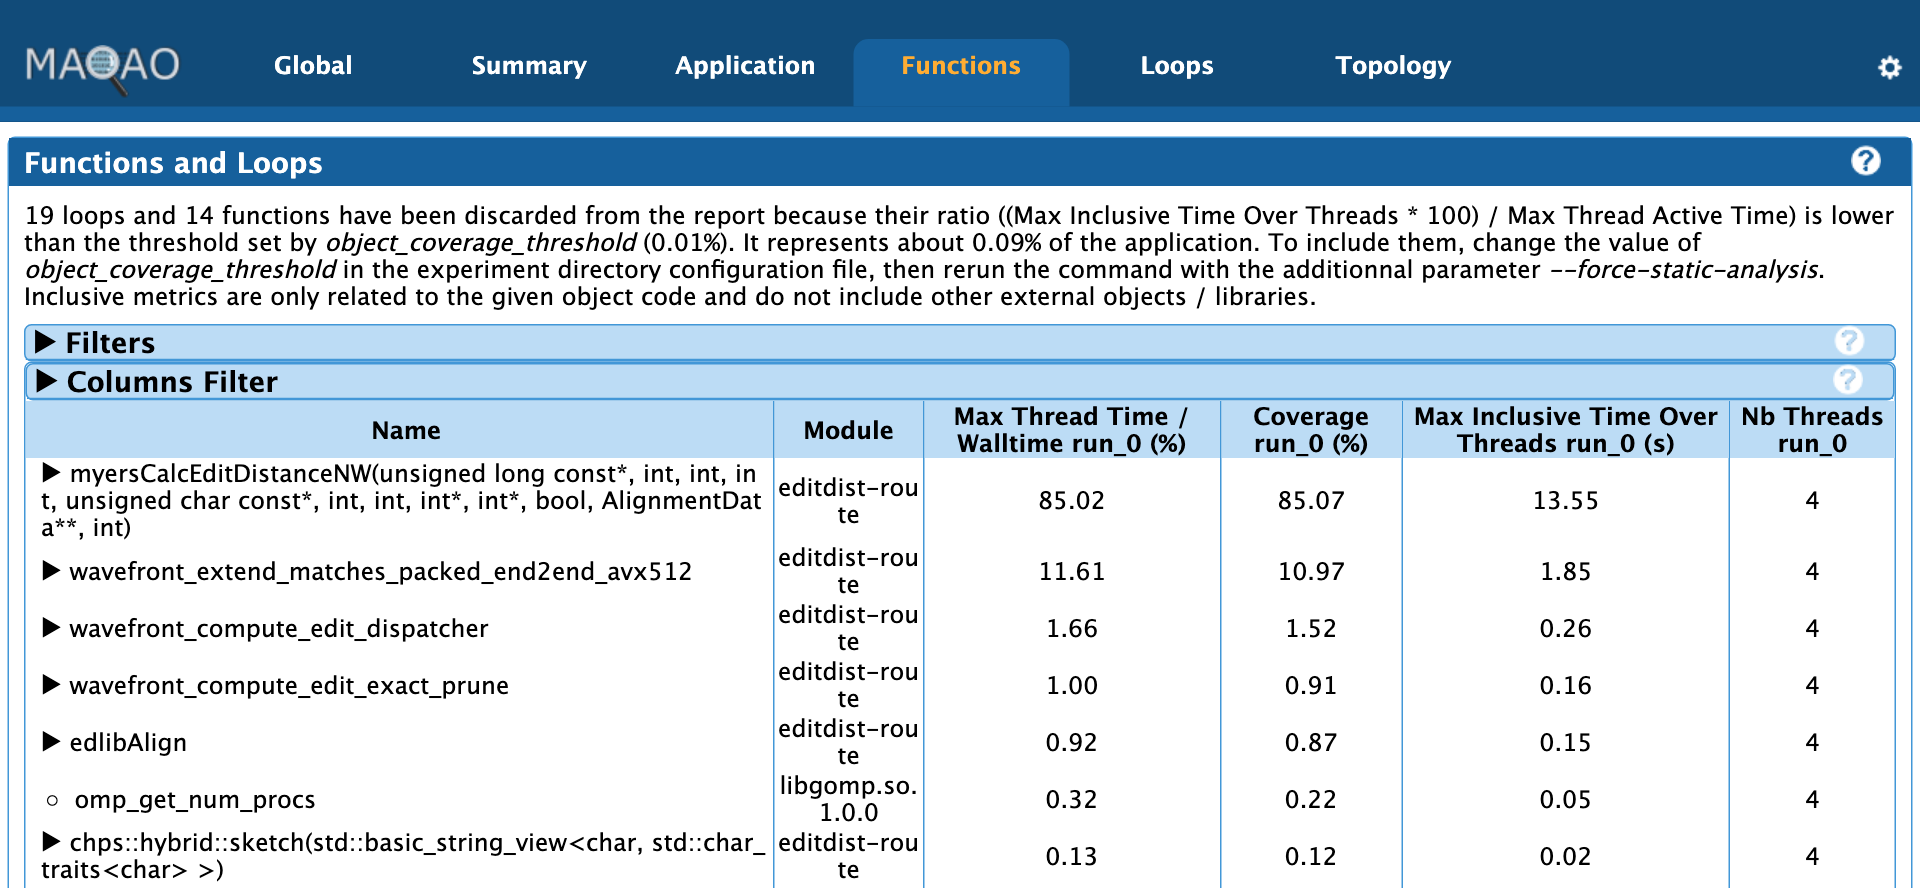
\includegraphics[width=.93\linewidth]{figures/maqao/fonctions-routage.png}
\sourcefig{bench/cpu/maqao/route.sbatch}\caption{Le profil des fonctions de MAQAO classe les routines pendant le calcul répété de la matrice de 2\,016 paires. La colonne \textit{Coverage} donne la part des échantillons de cycles.}\label{fig:maqao-route}
\end{figure}

\synthese{La règle de composition ramène le temps de \(2{,}433\pm0{,}016\)\,s avec Edlib seul à \(2{,}241\pm0{,}004\)\,s. Sur cette matrice, la réduction moyenne par bloc vaut 7,9\,\% (IC à 95\,\% de 7,4 à 8,4\,\%).}

\subsubsection{Structure des groupes dans les arbres de surveillance}
La cohorte comprend Wuhan-Hu-1~\cite{wuhanref} et neuf accessions par lignage pour sept lignages Pango~\cite{pango}. L’annexe~\ref{sec:accessions} donne les 64 identifiants versionnés et les décomptes de \texttt{N}. L’échantillonnage fixe l’effectif de chaque lignage indépendamment de sa fréquence dans la population. Le test cherche une arête qui isole exactement les neuf feuilles portant la même étiquette. Or la nomenclature Pango est hiérarchique~\cite{pango}. Le groupe étiqueté B.1 exclut notamment les feuilles étiquetées B.1.1.7, qui appartiennent à une de ses branches descendantes. Même dans un arbre fidèle à cette parenté, les neuf feuilles B.1 ne forment donc pas nécessairement un groupe exclusif. Dans un arbre enraciné, un groupe est retrouvé si les descendants d'une arête positive coïncident avec ses membres. Pour NJ, non enraciné, les deux côtés de l'arête sont examinés. Sur les 1\,905\,372 caractères lus, 65\,588 sont ambigus. La distance compte les différences entre caractères déposés, y compris aux positions ambiguës.
\chart{biology/phylogenie_surveillance.png}{Les distances globales entre paires et les groupes isolés par une arête sont comparés aux partitions de l'arbre de surveillance sur les identifiants communs.}{fig:surveillance}{scripts/phylogeny/phylo_groups.py}
À la figure~\ref{fig:surveillance}, la médiane est de 112 éditions pour les 252 paires de même lignage et de 402 pour les 1\,701 paires de lignages différents. Ces statistiques excluent les 63 paires contenant la référence. L'écart entre médianes est de 290 éditions. Lorsqu'on retire une accession et toutes ses paires, les 63 écarts vont de 282,5 à 295 éditions. Cette amplitude décrit la sensibilité au choix d'une feuille et conserve la dépendance entre paires qui partagent une accession. L’arbre public de l’UCSC du 23 novembre 2026~\cite{ushertree} contient 52 des 64 accessions, dont six du groupe A et aucune du groupe B.1.1.529. La méthode de placement par parcimonie de Turakhia et ses coauteurs~\cite{usher} attribue aux branches des longueurs en événements. Les chemins publics additionnent ces longueurs. Sur les 1\,326 paires de feuilles communes, la corrélation entre longueur de chemin et distance d’édition vaut \(r=0{,}124\). Plusieurs paires partagent une feuille. Le module Bio.Phylo de Biopython, présenté par Talevich et ses coauteurs~\cite{biophylo}, a relu le Newick et reproduit exactement les 1\,326 longueurs de chemin publiques.

\synthese{Sur les sept groupes de lignage, UPGMA en isole deux et NJ trois. Parmi les 27 bipartitions internes de longueur positive de l’arbre UShER restreint aux 52 feuilles communes, UPGMA en retrouve six et NJ huit.}
